\subsection{Example Section}

Lorem ipsum dolor sit amet, consectetur adipiscing elit,
sed do eiusmod tempor incididunt ut labore et dolore magna aliqua. Ut enim ad
minim veniam, quis nostrud exercitation ullamco laboris nisi ut aliquip ex ea
commodo consequat. Duis aute irure dolor in reprehenderit in voluptate velit
esse cillum dolore eu fugiat nulla pariatur. Excepteur sint occaecat cupidatat
non proident, sunt in culpa qui officia deserunt mollit anim id est laborum.

\ignore{this is an example longform comment}

\subsection{Another Example Section}

You can site papers by putting there bibtex in the sources. bib file in the latex
folder. Most bibtex can be found on the cite where the paper is. The paper will not
compile if there are no sources. You can site by just doing \texttt{\\cite\{nameofsource\}},
I have already added the two sources included in the doc folder \cite{behaviortrees}\cite{pound}.

\subsection{Adding figures}

You can add figures with captions:

\begin{figure}[H]
  \centering
    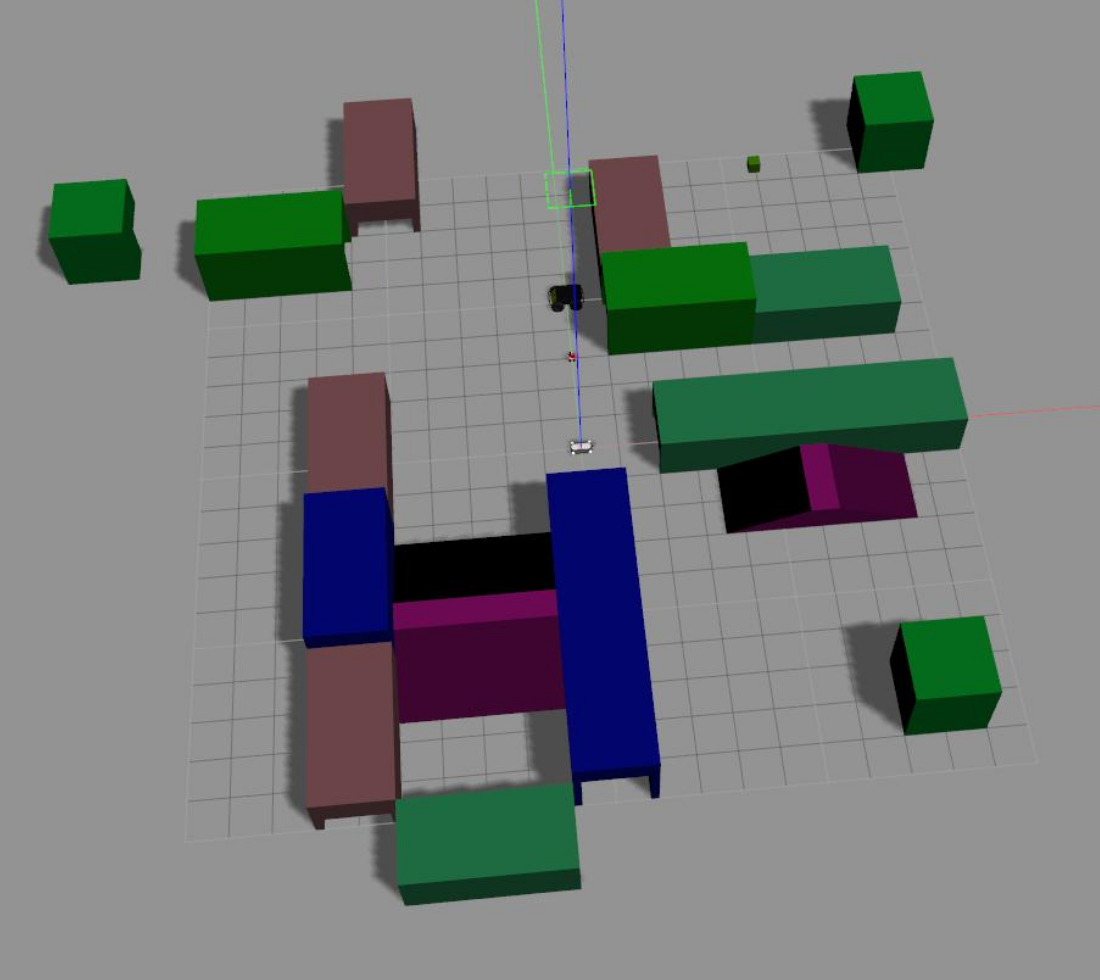
\includegraphics[width=0.5\textwidth]{map2}
  \caption{This is a caption of this figure.}
  \label{fig:something1}
\end{figure}

\begin{figure}[H]
  \centering
    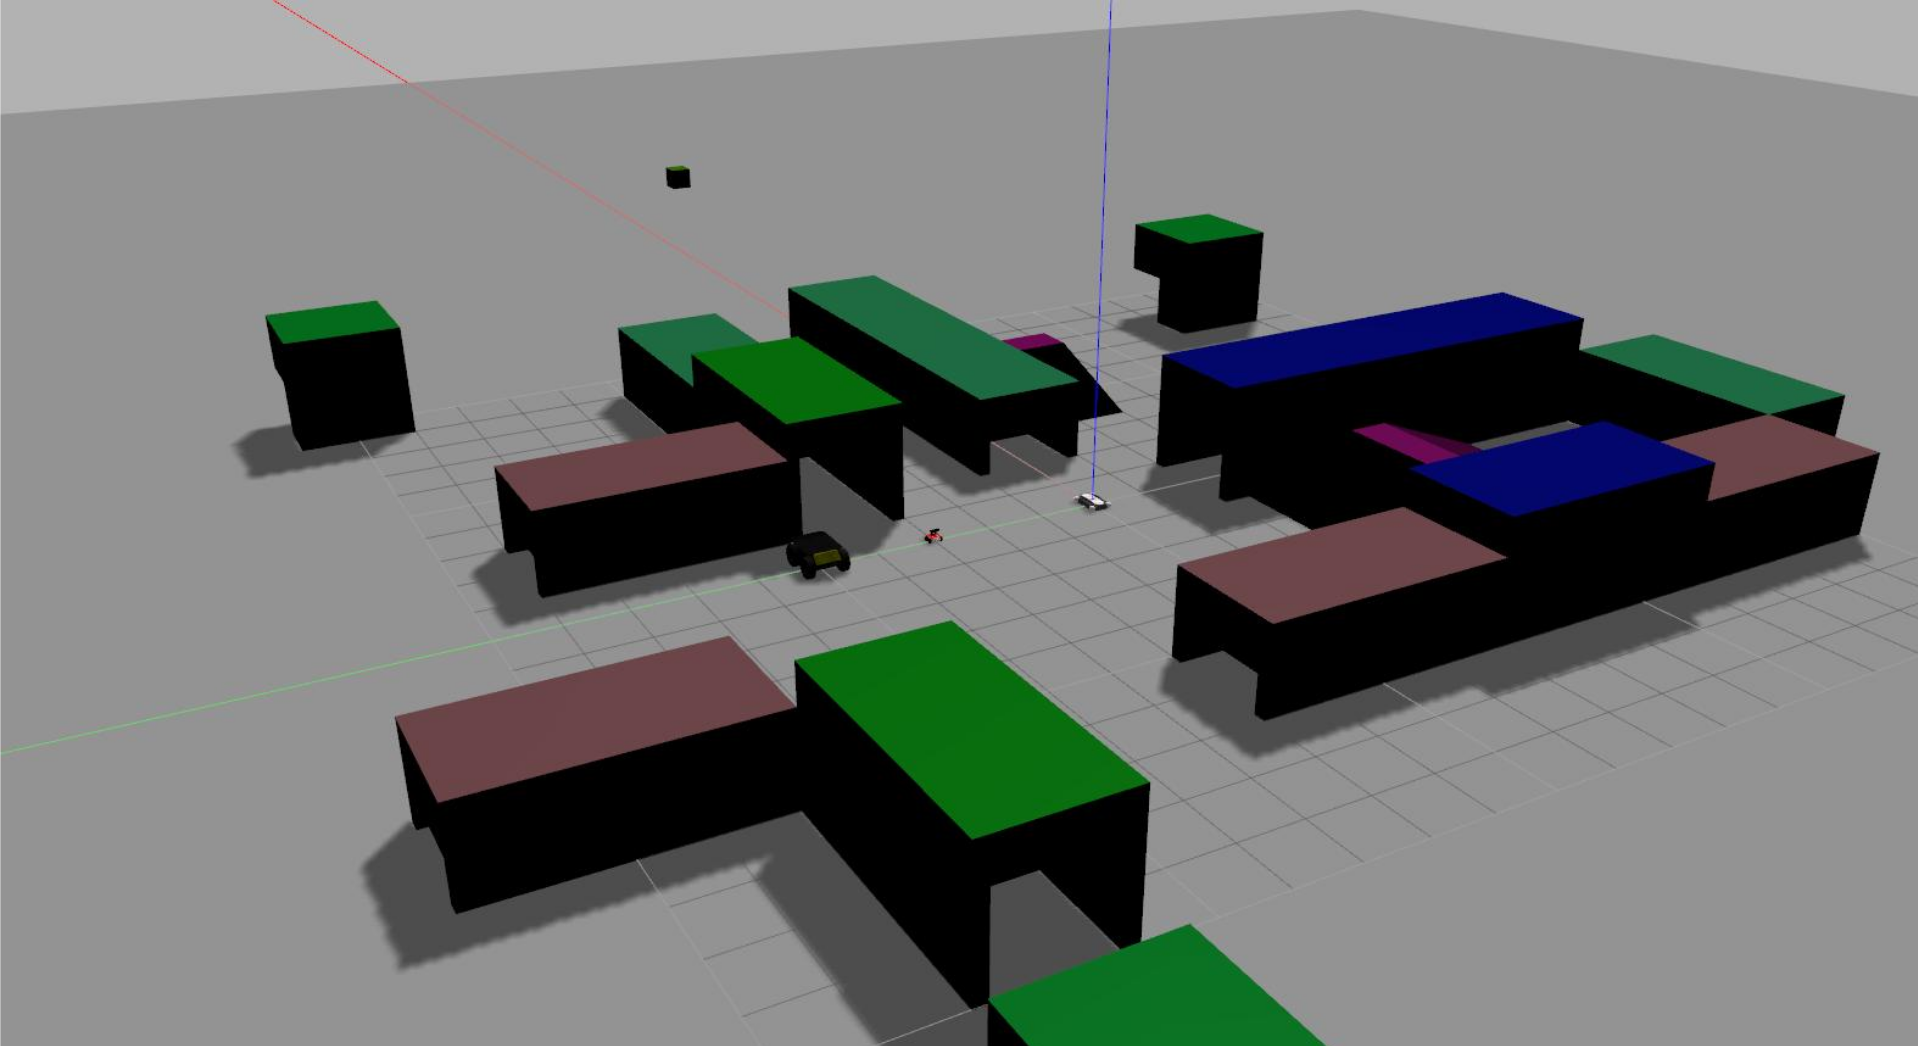
\includegraphics[width=0.5\textwidth]{map1}
  \caption{This is a caption of this figure.}
  \label{fig:something2}
\end{figure}

Lorem ipsum dolor sit amet, consectetur adipiscing elit,
sed do eiusmod tempor incididunt ut labore et dolore magna aliqua. Ut enim ad
minim veniam, quis nostrud exercitation ullamco laboris nisi ut aliquip ex ea
commodo consequat. Duis aute irure dolor in reprehenderit in voluptate velit
esse cillum dolore eu fugiat nulla pariatur. Excepteur sint occaecat cupidatat
non proident, sunt in culpa qui officia deserunt mollit anim id est laborum.

\begin{figure}[H]
  \centering
    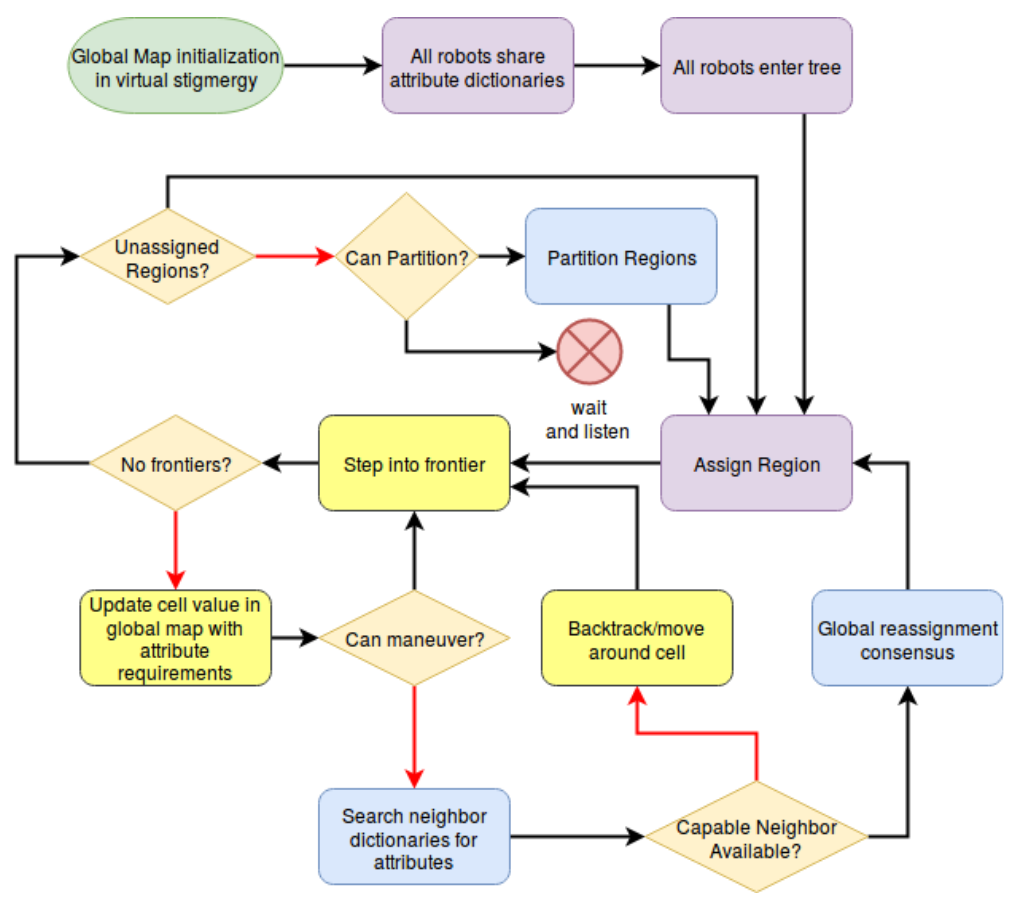
\includegraphics[width=0.5\textwidth]{diagram1}
  \caption{This is a caption of this figure.}
  \label{fig:something3}
\end{figure}

\begin{figure}[H]
  \centering
    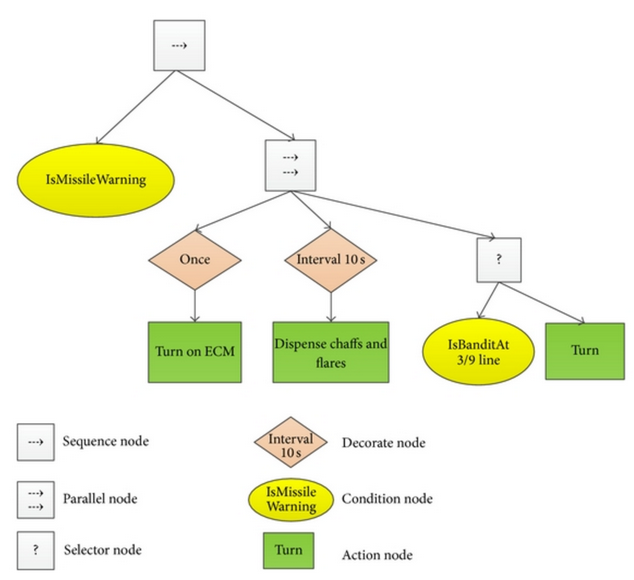
\includegraphics[width=0.5\textwidth]{diagram2}
  \caption{This is a caption of this figure.}
  \label{fig:something4}
\end{figure}

Lorem ipsum dolor sit amet, consectetur adipiscing elit,
sed do eiusmod tempor incididunt ut labore et dolore magna aliqua. Ut enim ad
minim veniam, quis nostrud exercitation ullamco laboris nisi ut aliquip ex ea
commodo consequat. Duis aute irure dolor in reprehenderit in voluptate velit
esse cillum dolore eu fugiat nulla pariatur. Excepteur sint occaecat cupidatat
non proident, sunt in culpa qui officia deserunt mollit anim id est laborum.

% this section has 3 figures together

\begin{figure}
    \centering
    \begin{subfigure}[b]{0.15\textwidth}
        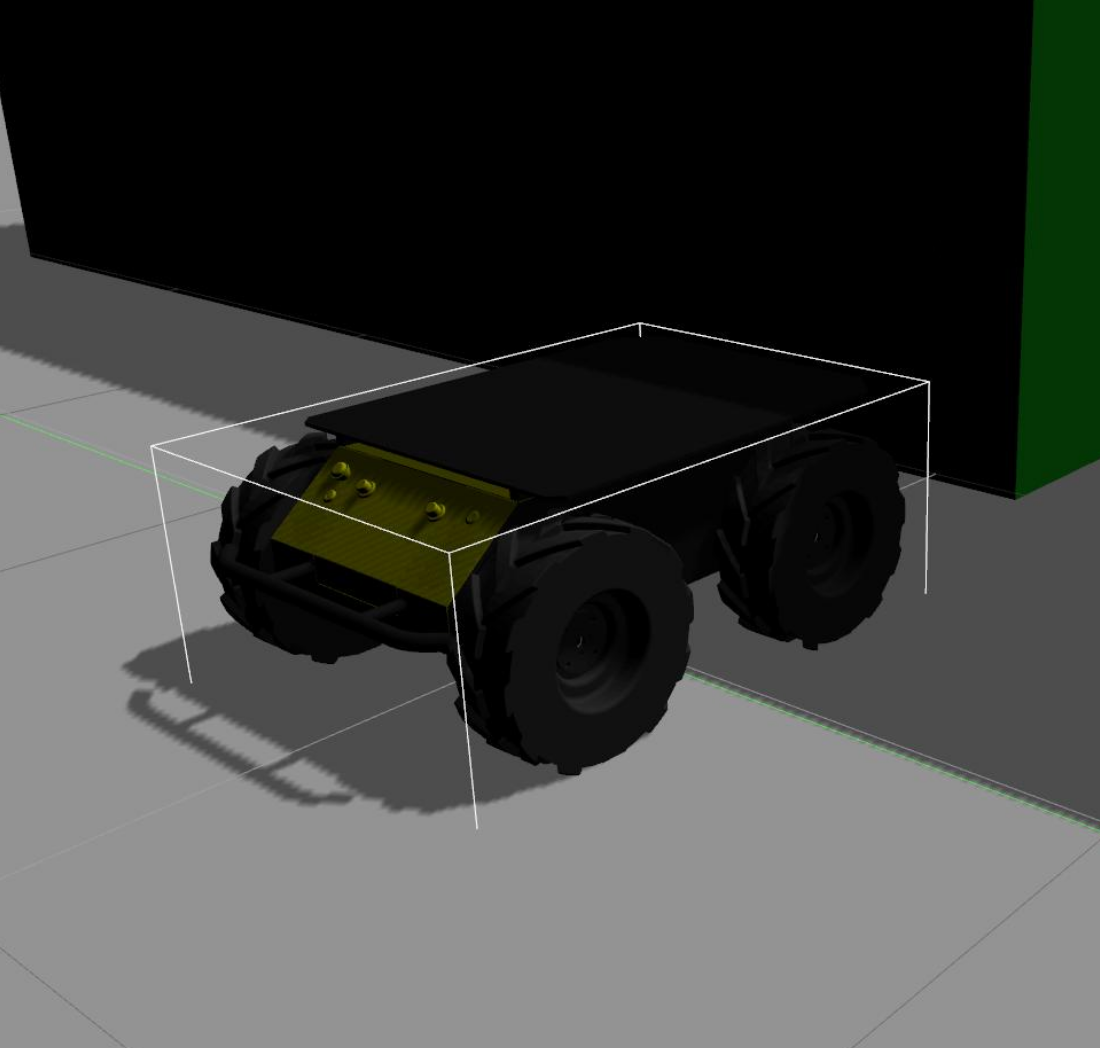
\includegraphics[width=\textwidth]{bot1}
        \caption{A gull}
        \label{fig:bot1}
    \end{subfigure}
    \begin{subfigure}[b]{0.15\textwidth}
        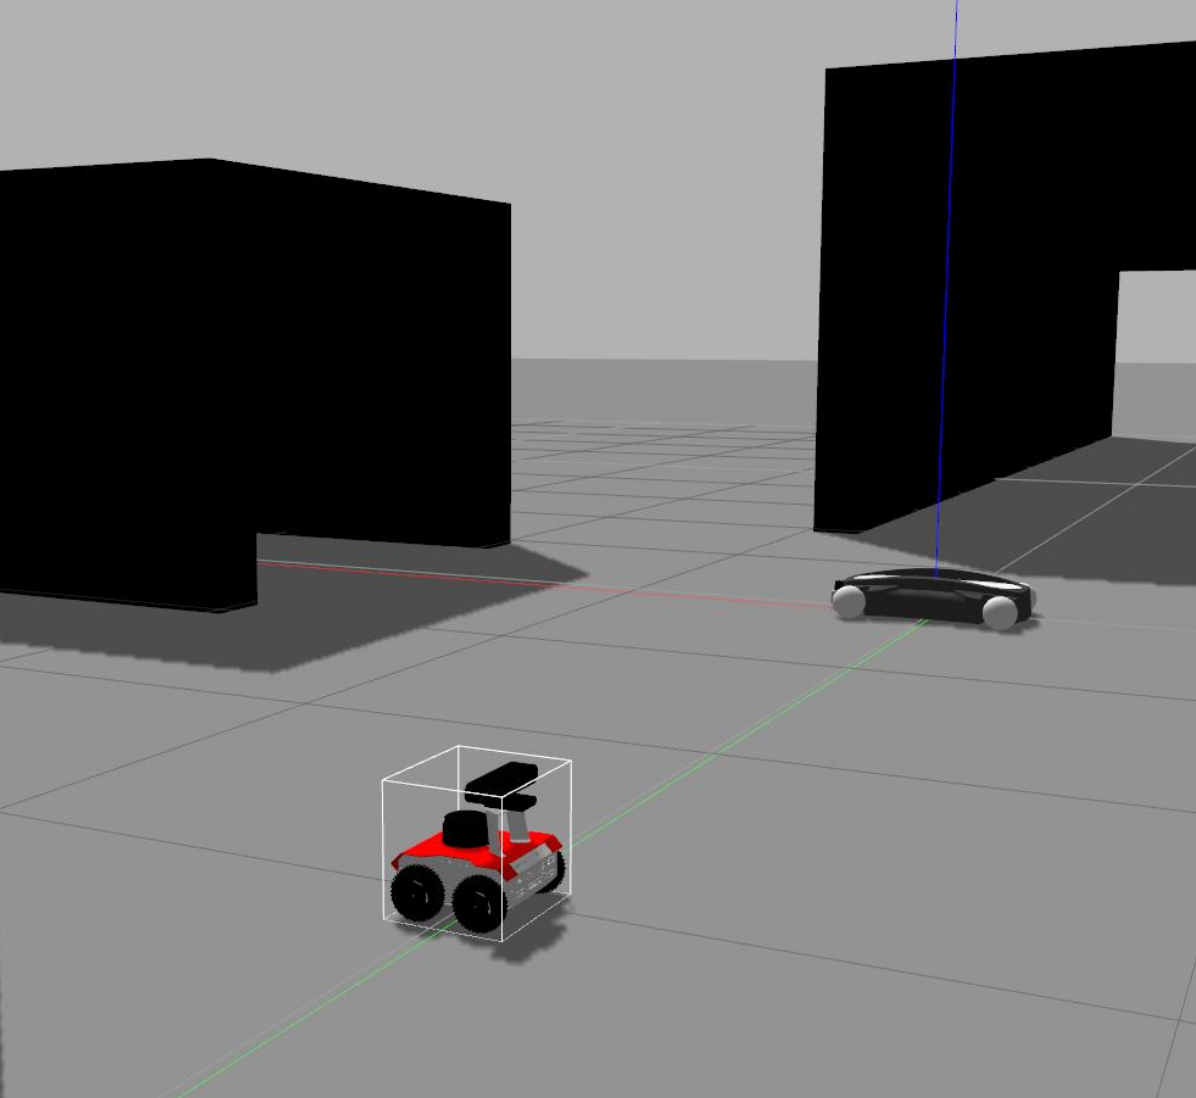
\includegraphics[width=\textwidth]{bot2}
        \caption{A tiger}
        \label{fig:bot2}
    \end{subfigure}
    \begin{subfigure}[b]{0.15\textwidth}
        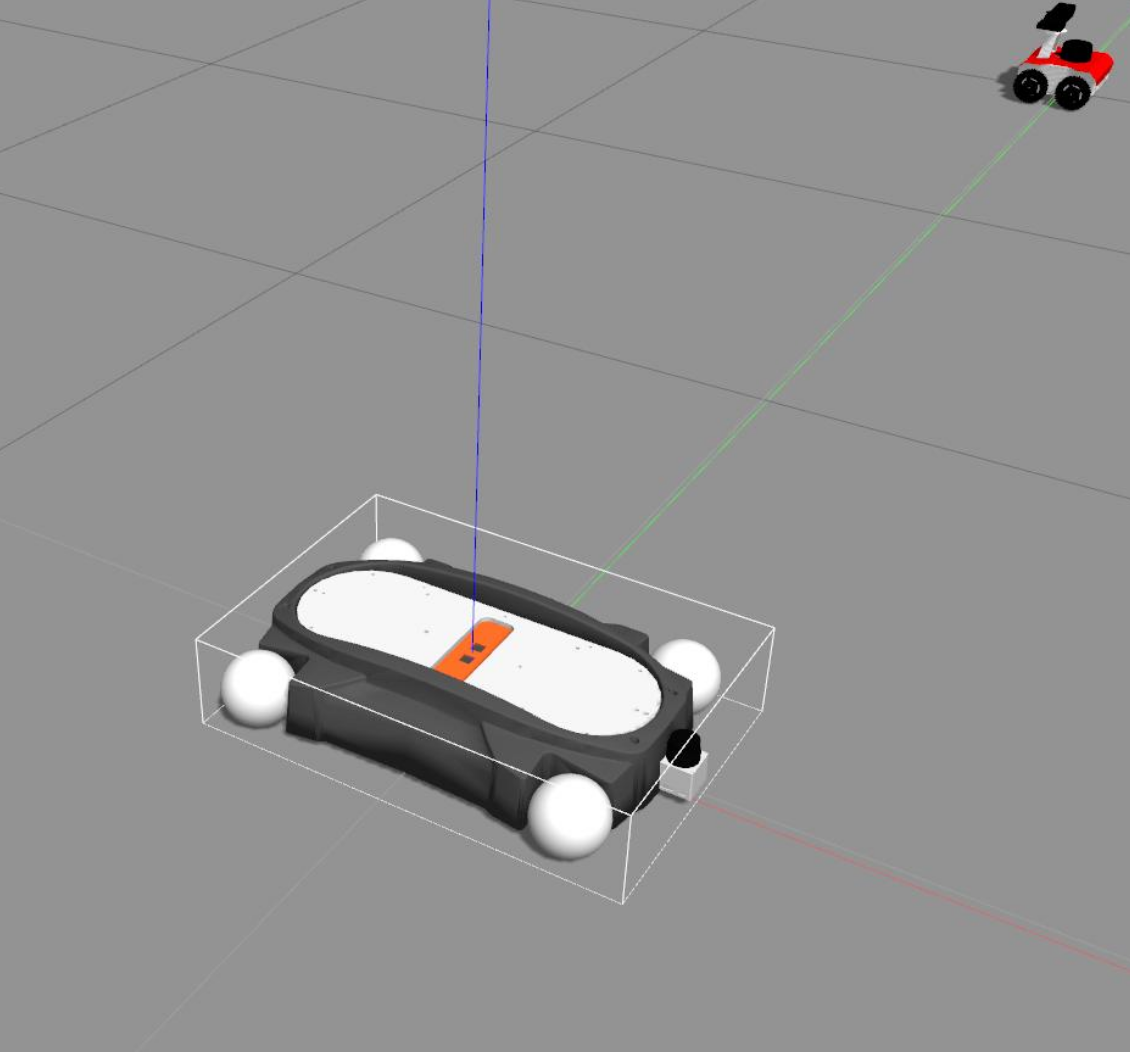
\includegraphics[width=\textwidth]{bot3}
        \caption{A mouse}
        \label{fig:bot3}
    \end{subfigure}
    \caption{Observe our future overlords}\label{fig:bots}
\end{figure}
